\documentclass[11pt]{article}
% =============================================================================
% preamble.tex — shared LaTeX preamble for the Pagesmith guides.
% \input this from each guide's .tex. Verified to compile with pdflatex (TeX Live).
% =============================================================================
\usepackage[margin=1in]{geometry}
\usepackage{amsmath,amssymb}
\usepackage{microtype}
\usepackage{enumitem}
\usepackage{xcolor}
\usepackage{hyperref}
\usepackage{listings}
\usepackage{tikz}
\usetikzlibrary{positioning,arrows.meta,shapes.geometric,calc,fit,backgrounds}
\usepackage{placeins}   % \FloatBarrier
\usepackage{caption}
\captionsetup{font=small,skip=8pt}

\hypersetup{colorlinks=true,linkcolor=blue!55!black,urlcolor=blue!55!black,citecolor=blue!55!black}

% A bit of breathing room around floats.
\setlength{\textfloatsep}{16pt plus 4pt minus 4pt}
\setlength{\intextsep}{16pt plus 4pt minus 4pt}

% ---- code listings ----------------------------------------------------------
\definecolor{codebg}{RGB}{248,248,248}
\definecolor{codecmt}{RGB}{0,128,0}
\definecolor{codestr}{RGB}{170,55,0}
\definecolor{codekw}{RGB}{0,0,180}
% No fixed `language=` (so neither JS nor JSON trips listings' keyword parser);
% code is shown as clean monospace in a framed, tinted box.
\lstset{
  basicstyle=\ttfamily\small,
  backgroundcolor=\color{codebg},
  commentstyle=\color{codecmt}\itshape,
  stringstyle=\color{codestr},
  showstringspaces=false,
  breaklines=true,
  columns=fullflexible,
  keepspaces=true,
  frame=single,
  framesep=4pt,
  rulecolor=\color{black!20},
  aboveskip=10pt,
  belowskip=6pt
}

% ---- tikz diagram helpers (boxes + arrows) ----------------------------------
\definecolor{boxblue}{RGB}{79,124,255}
\definecolor{boxgray}{RGB}{90,98,112}
\tikzset{
  box/.style   = {draw, rounded corners, align=center, font=\small, inner sep=6pt, fill=boxblue!8, draw=boxblue!60},
  gbox/.style  = {draw, rounded corners, align=center, font=\small, inner sep=6pt, fill=black!4, draw=black!35},
  flow/.style  = {-{Stealth[length=2.4mm]}, thick, draw=boxgray},
}

% ---- convenience macros -----------------------------------------------------
\newcommand{\code}[1]{\texttt{#1}}


\title{Pagesmith --- The Editor Internals\\[2pt]\large A Developer Guide to \texttt{edit-mode.js}}
\author{David Falk}
\date{}

\begin{document}
\maketitle

\begin{abstract}
\noindent This guide explains how Pagesmith's inline content editor
(\code{edit-mode.js}) is \emph{built}, for developers who maintain or extend it.
We follow the file's own \textsc{surface map}: how it boots and gates itself off
production, the state model that survives the constant save\,$\to$\,reload cycle,
the \code{data-edit-*} binding protocol that lets parts become editable with zero
editor code, the true-index trick that keeps list reordering correct, the
Sections panel as a staging editor, the save/publish/revert backend, and the
media upload pipeline. It closes with a recipe section for extending the editor
and a catalogue of sharp edges to respect. Pagesmith is a generic, JSON-driven
page builder; nothing here is specific to any one site.
\end{abstract}

\tableofcontents
\bigskip

%==============================================================================
\section{Orientation: what edit-mode.js is}
%==============================================================================

\code{edit-mode.js} is a single $\sim$2250-line IIFE that turns an ordinary live
web page into an editable surface. It belongs to an engine/instance split: the
\emph{engine} (skeleton, catalogue of parts, and editor) is brand-neutral and
renders whatever typed blocks are in a page's JSON; the \emph{instance} is one
config file (\code{site-config.js}, exposed as \code{window.SITE}) plus content
JSON, CSS, and HTML shells.

The editor ships no site-specific strings. Everything it needs about \emph{this}
deployment --- prod hostnames, wordmark, media-picker tabs, full-quality folders,
friendly page names --- arrives through \code{window.SITE}. Keep it that way:
route anything site-shaped through config rather than hardcoding it.

The file opens with a \textsc{surface map} comment that is the canonical table of
contents for the code. Two gotchas, also called out at the top of the file,
explain a great deal of what follows:

\begin{enumerate}[leftmargin=1.5em]
  \item \textbf{The Sections panel is a staging editor.} Add / hide / delete /
  reorder are staged inside the panel and only written to the live page on
  \emph{Apply \& Save}. The on-page section count does not change as you click.
  \item \textbf{Many ``Done'' buttons call \code{save(true)}, which reloads the
  page.} After most edits the page reloads and re-renders from the saved model.
  That is \emph{why} unsaved inline edits live in \code{state.models}, not in the
  DOM --- the DOM is disposable.
\end{enumerate}

%==============================================================================
\section{Boot \& gating}
%==============================================================================

\subsection{Two gates, by design}

\code{edit-mode.js} is not a static \code{<script>} tag. It is injected at
runtime by \code{media-base.js}, and \emph{only on non-prod hosts}:

\begin{lstlisting}
// media-base.js
var isProdHost = !!(window.SITE && window.SITE.isProd(host));
// Load the inline editor runtime on dev/local hosts only (never on prod).
// edit-mode.js self-gates further: no-ops unless /.auth/me has the editor role.
if (!isProdHost) {
  var es = document.createElement('script');
  es.src = '/javascript/edit-mode.js';
  es.defer = true;
  (document.head || document.documentElement).appendChild(es);
}
\end{lstlisting}

So there are two independent gates (defence in depth), plus a third belt-and-braces
check inside the file itself:

\begin{lstlisting}
var host = (location.hostname || '').toLowerCase();
if (window.SITE && window.SITE.isProd(host)) return; // never on the live site
\end{lstlisting}

\begin{itemize}[leftmargin=1.5em]
  \item \textbf{Host gate} (media-base): on a prod host the editor is never even
  downloaded --- production users pay zero bytes for it.
  \item \textbf{Self-gate} (top of file): refuses to run if mistakenly placed on a
  prod page.
  \item \textbf{Role gate} (\code{boot}): even when loaded, does nothing unless
  the signed-in principal carries the \code{editor} role.
\end{itemize}

\subsection{The role gate in \texttt{boot()}}

\begin{lstlisting}
function boot() {
  fetch('/.auth/me').then(r => r.ok ? r.json() : null).then(function (me) {
    var p = me && me.clientPrincipal;
    state.principal = p;
    var roles = (p && p.userRoles) || [];
    if (roles.indexOf('editor') === -1) {
      console.info('[engine-edit] not an editor - editor disabled.');
      return;                          // everything below never runs
    }
    /* build toolbar, wire events, expose window.EngineEdit */
  });
}
\end{lstlisting}

\code{/.auth/me} is the Azure Static Web Apps endpoint returning the current
\code{clientPrincipal} (provider, user id, roles). Anonymous or non-editor users
get a page indistinguishable from the public site.

Why fetch roles client-side if the server enforces them anyway? Because the client
gate is purely cosmetic --- it decides whether to \emph{show} editing UI. Every
mutating API call is independently enforced server-side via \code{requireEditor}
(\S\ref{sec:backend}). A forged client check still bounces off the Functions.

\begin{figure}[h]
\centering
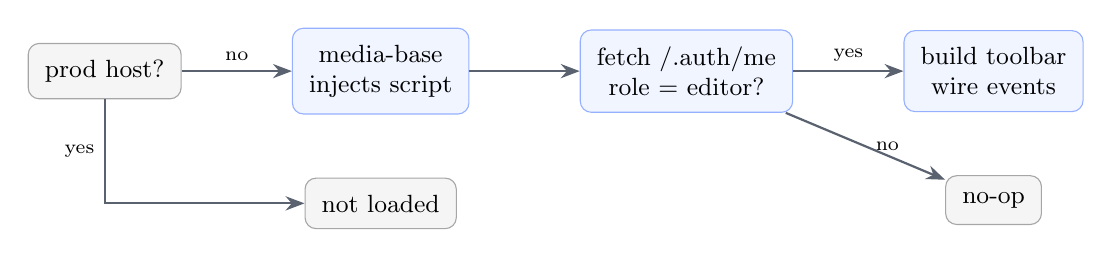
\begin{tikzpicture}[node distance=8mm and 14mm]
  \node[gbox] (host)  {prod host?};
  \node[box, right=of host] (load) {media-base \\ injects script};
  \node[box, right=of load] (role) {fetch /.auth/me \\ role = editor?};
  \node[box, right=of role] (run)  {build toolbar \\ wire events};
  \node[gbox, below=of load] (none1) {not loaded};
  \node[gbox, below=of run]  (none2) {no-op};
  \draw[flow] (host) -- node[above,font=\scriptsize]{no} (load);
  \draw[flow] (host) |- node[pos=0.25,left,font=\scriptsize]{yes} (none1);
  \draw[flow] (load) -- (role);
  \draw[flow] (role) -- node[above,font=\scriptsize]{yes} (run);
  \draw[flow] (role) -- node[pos=0.5,right,font=\scriptsize]{no} (none2);
\end{tikzpicture}
\caption{The three gates: host (no download), self-gate, and role.}
\end{figure}

\subsection{The rest of boot}

Past the gate, \code{boot()} does the housekeeping that lets the editor feel
continuous across the constant reloads: it restores \code{state.editing} and
scroll position from \code{sessionStorage}, builds the toolbar, wires the
\code{engine-data-ready} and \code{engine-rebind} listeners, adds a
\code{beforeunload} dirty-guard, and exposes \code{window.EngineEdit}. The
\code{engine-data-ready} listener is the heart of the data flow (\S\ref{sec:state}).

%==============================================================================
\section{The state model}\label{sec:state}
%==============================================================================

Everything the editor knows lives in one object:

\begin{lstlisting}
var state = {
  file: null,      // primary page file key, e.g. 'page-music' (toolbar pill)
  data: null,      // primary page model - a POINTER into models[file]
  models: {},      // fileKey -> data   (the page file AND 'global')
  dirtyFiles: {},  // fileKey -> true   (which models have unsaved edits)
  editing: false,  // Edit vs Preview
  principal: null  // the SWA clientPrincipal from /.auth/me
};
\end{lstlisting}

\subsection{Two models, and the \texttt{fileKeyOf} router}

A rendered page is assembled from two JSON files: the \textbf{page file}
(\code{index.json}, \code{page-music.json}, \dots) holding the page's own blocks,
and \textbf{\code{global.json}} holding the chrome shared by every page (nav,
social, footer, questionnaire, tracking, theme). The header and footer are
editable on every page but belong to \code{global}, not to the page you are on.
So each editable node declares \emph{which model it edits} via \code{data-edit-file}:

\begin{lstlisting}
function fileKeyOf(node) {
  var a = node && node.closest && node.closest('[data-edit-file]');
  return (a && a.getAttribute('data-edit-file')) || state.file;
}
function modelOf(node) { return state.models[fileKeyOf(node)]; }
\end{lstlisting}

The rule: a node inside a \code{[data-edit-file="global"]} ancestor edits the
global model; everything else defaults to the current page file. This is the most
important routing decision in the editor --- get it wrong and a header edit
silently lands in the page model and is lost on the next page.

\begin{figure}[h]
\centering
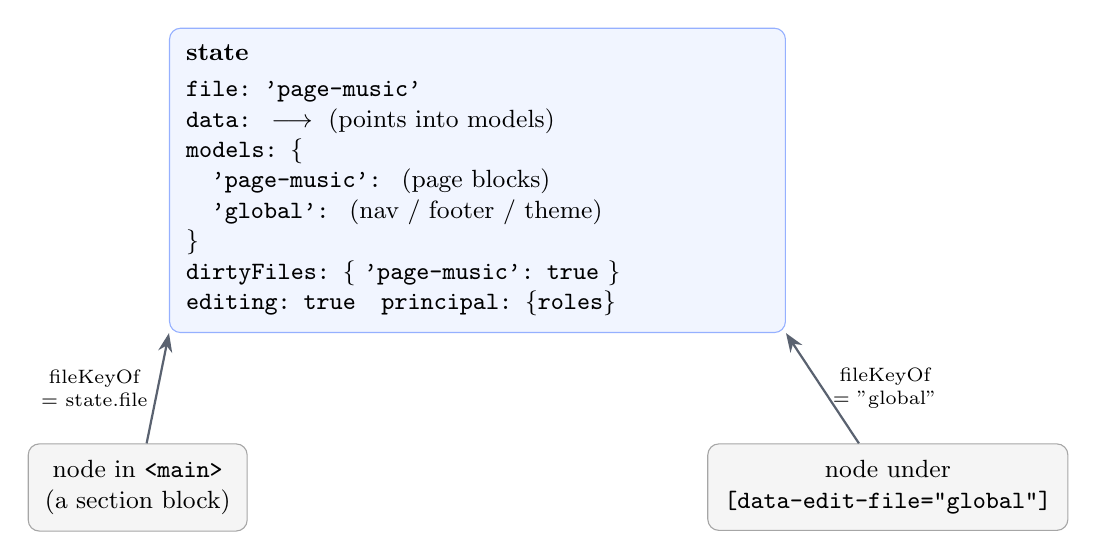
\begin{tikzpicture}[node distance=6mm]
  \node[box, align=left, text width=7.4cm] (state) {
    \textbf{state}\\[2pt]
    \code{file: 'page-music'}\\
    \code{data:} \;$\longrightarrow$\; (points into models)\\
    \code{models: \{}\\
    \quad \code{'page-music':}\; (page blocks)\\
    \quad \code{'global':}\; (nav / footer / theme)\\
    \code{\}}\\
    \code{dirtyFiles: \{ 'page-music': true \}}\\
    \code{editing: true}\quad \code{principal: \{roles\}}
  };
  \node[gbox, below left=14mm and -1cm of state] (n1) {node in \code{<main>}\\(a section block)};
  \node[gbox, below right=14mm and -1cm of state] (n2) {node under\\\code{[data-edit-file="global"]}};
  \draw[flow] (n1) -- node[left,font=\scriptsize,align=center]{fileKeyOf\\= state.file} (state.south west);
  \draw[flow] (n2) -- node[right,font=\scriptsize,align=center]{fileKeyOf\\= "global"} (state.south east);
\end{tikzpicture}
\caption{\code{fileKeyOf(node)} routes each node to its backing model.}
\end{figure}

\code{state.data} and \code{state.file} are conveniences that track the current
page; \code{state.models} is the source of truth.

\subsection{Populating models: \texttt{onData}}

The skeleton loads each JSON file and announces it; the editor folds it in:

\begin{lstlisting}
window.__ENGINE_DATA__ = { file, data };
document.dispatchEvent(new CustomEvent('engine-data-ready',
                                       { detail: { file, data } }));

function onData(file, data) {
  state.models[file] = data;
  if (file !== 'global') { state.file = file; state.data = data; }
  bindAll(); refreshToolbar();
  /* restore scroll after a save->reload if pendingScroll is set */
}
\end{lstlisting}

The \code{file !== 'global'} guard ensures the global model never clobbers the
page pointers. Both models may arrive in either order, so \code{boot()} replays a
global payload (\code{\_\_ENGINE\_GLOBAL\_\_}) that raced ahead.

\subsection{Dirty tracking}

\begin{lstlisting}
function isDirty() { return Object.keys(state.dirtyFiles).length > 0; }
function markDirty(fk) { if (fk) state.dirtyFiles[fk] = true; refreshToolbar(); }
\end{lstlisting}

Every mutation calls \code{markDirty(fileKeyOf(node))}; the toolbar reflects it.
\code{save()} clears \code{dirtyFiles} only after the POSTs succeed.

%==============================================================================
\section{The data-edit-* binding protocol}
%==============================================================================

The editor does not know your blocks' data shapes. Parts \emph{tag} their DOM
with \code{data-edit-*} attributes, and the editor wires behaviour onto whatever
it finds. This is the entire contract between a part and the editor.

\begin{center}\small
\begin{tabular}{@{}p{4.4cm}p{8.2cm}@{}}
\hline
\textbf{Attribute} & \textbf{Behaviour} \\
\hline
\code{data-edit-text="path"} & inline plain-text (\code{contentEditable}); writes \code{textContent} \\
\code{data-edit-html="path"} & inline rich text; writes \code{innerHTML} \\
\code{data-edit-image="path"} & click $\to$ media picker / section editor \\
\code{data-edit-attr="path|attr"} & click $\to$ \code{prompt()} edits one attribute \\
\code{data-edit-bg="blob"} & click $\to$ replace a fixed CSS background blob \\
\code{data-edit-list="path"} & drag-reorder + the list panel \\
\code{data-edit-file="key"} & routes all of the above to a model \\
\code{data-item-index="i"} & on each LIST CHILD, its true array index \\
\hline
\end{tabular}
\end{center}

\subsection{\texttt{bindAll()} --- idempotent, after every render}

\begin{lstlisting}
function bindAll() {
  if (!Object.keys(state.models).length) return;
  document.querySelectorAll('[data-edit-text]').forEach(n => bindText(n, false));
  document.querySelectorAll('[data-edit-html]').forEach(n => bindText(n, true));
  document.querySelectorAll('[data-edit-image]').forEach(bindImage);
  document.querySelectorAll('[data-edit-attr]').forEach(bindAttr);
  document.querySelectorAll('[data-edit-bg]').forEach(bindBg);
  document.querySelectorAll('[data-edit-list]').forEach(bindList);
  setEditing(state.editing);
}
\end{lstlisting}

\code{bindAll()} runs after each (re)render --- from \code{onData} and from the
\code{engine-rebind} event a part fires after re-rendering itself. It must be
idempotent, so each binder guards with a per-node flag:

\begin{lstlisting}
function bindText(n, isHtml) {
  if (n.__engineBound) return; n.__engineBound = true; // bind once
  /* ... */
}
\end{lstlisting}

This is why \code{bindAll()} can be called freely after any partial re-render
without stacking duplicate listeners. When you add a new binder (\S\ref{sec:extend}),
keep the \code{\_\_engineBound} guard --- it is load-bearing.

\subsection{Paths: tokenize then resolve}

The glue between a node and the model is a path string like
\code{sections[2].items[0].value}. Two functions do all the addressing:

\begin{lstlisting}
function tokenize(path) {
  return String(path)
    .replace(/\[(\d+)\]/g, '.$1')   // sections[2] -> sections.2
    .split('.')
    .filter(s => s !== '');
}
function getByPath(obj, path) {
  var t = tokenize(path), o = obj;
  for (var i = 0; i < t.length; i++) { if (o == null) return undefined; o = o[t[i]]; }
  return o;
}
function setByPath(obj, path, val) {
  var t = tokenize(path), o = obj;
  for (var i = 0; i < t.length - 1; i++) {
    var k = t[i];
    // create the missing container: array if the NEXT token is numeric, else object
    if (o[k] == null || typeof o[k] !== 'object')
      o[k] = /^\d+$/.test(t[i + 1]) ? [] : {};
    o = o[k];
  }
  o[t[t.length - 1]] = val;
}
\end{lstlisting}

\textbf{Worked example.} \code{sections[2].items[0].value} tokenizes to
\code{['sections','2','items','0','value']}. Against:

\begin{lstlisting}
{
  "sections": [
    { "type": "heading", "text": "Hi" },
    { "type": "text", "body": "..." },
    { "type": "links", "items": [ { "value": "https://a", "label": "A" } ] }
  ]
}
\end{lstlisting}

\code{getByPath} walks \code{model}\,$\to$\,\code{sections}\,$\to$\,\code{[2]}\,$\to$\,%
\code{items}\,$\to$\,\code{[0]}\,$\to$\,\code{value} and returns \code{"https://a"}.
\code{setByPath} walks the same route but stops one short, then assigns. Its
auto-vivify rule (array when the next token is numeric, else object) lets a part
bind to a path that does not exist yet --- the first edit materialises the
container correctly.

\subsection{Text/HTML, image, attr, bg}

Text binding writes through on \code{input}:

\begin{lstlisting}
n.addEventListener('input', function () {
  var m = modelOf(n); if (!m) return;
  setByPath(m, n.getAttribute(isHtml ? 'data-edit-html' : 'data-edit-text'),
            isHtml ? n.innerHTML : n.textContent);
  markDirty(fileKeyOf(n));
});
\end{lstlisting}

Plain text intercepts Enter to blur; rich text stores raw \code{innerHTML} (a
sharp edge, \S\ref{sec:edges}). \textbf{image} clicks open the section's unified
Edit panel (or, for legacy standalone media, a floating Replace/Remove toolbar);
\code{replaceMedia} opens the picker, writes the chosen path with \code{setByPath},
repaints in place, and marks dirty. \textbf{attr} splits \code{path|attr}, prompts,
and writes both model and live attribute. \textbf{bg} names a fixed blob and
replaces its bytes at that exact filename.

%==============================================================================
\section{List reordering: the data-item-index contract}\label{sec:list}
%==============================================================================

On-page drag-to-reorder hides a subtle, expensive bug class, and the editor avoids
it deliberately.

\subsection{The bug class}

A list block renders DOM children from a backing array --- but a part may render
\emph{fewer} children than the array has items (it might skip a blank URL or an
invalid image). Now array index and DOM position have desynced. If reorder spliced
by DOM position, it would move the \emph{wrong} array element whenever an earlier
item was filtered out: the visible order changes, but a different, invisible item
actually moved. Silent corruption.

\subsection{The fix: stamp the true index}

Each list part stamps every rendered child with its true array index via
\code{data-item-index} (documented in the \code{blocks.js} editing protocol):

\begin{lstlisting}
// blocks.js - a gallery part stamping the real array index j on each child
var img = ctx.el('img', { src: ctx.mediaUrl(src), alt: (im && im.alt) || '',
                          'data-item-index': j /* TRUE index */ });
\end{lstlisting}

The editor prefers the stamp over DOM position, falling back only when absent:

\begin{lstlisting}
function itemIndexOf(container, child) {
  if (child && child.getAttribute) {
    var raw = child.getAttribute('data-item-index');
    if (raw != null && raw !== '') { var n = parseInt(raw, 10); if (!isNaN(n)) return n; }
  }
  return Array.prototype.indexOf.call(container.children, child); // fallback
}
\end{lstlisting}

The DOM-position fallback exists for simple one-child-per-item lists, but
\textbf{any part that filters items must stamp}, or it reintroduces the desync.
That is the rule when authoring a part.

\subsection{The splice}

\code{startReorder} and \code{dragover} record \emph{true} indices; \code{endReorder}
splices the model and saves:

\begin{lstlisting}
function endReorder() {
  var d = dragNow; dragNow = null;
  if (d && d.to != null && d.to !== d.from) {
    var fk = fileKeyOf(d.container), model = state.models[fk];
    var arr = getByPath(model, d.path);
    if (Array.isArray(arr) && d.from < arr.length) {
      arr.splice(d.to, 0, arr.splice(d.from, 1)[0]); // move from -> to
      markDirty(fk);
      save(true);                                     // persist + reload
    }
  }
}
\end{lstlisting}

Because \code{from} and \code{to} are true array indices, the splice is correct
even when DOM and array disagree on length.

%==============================================================================
\section{The Sections panel as a staging editor}\label{sec:sections}
%==============================================================================

\code{openSectionsNav()} edits page structure --- reorder, hide/show, delete, jump,
edit. The crucial design choice: it edits a \emph{working copy}, not the live page.
Nothing changes the on-page section count until \emph{Apply \& Save}.

\subsection{The working list}

It assembles one flat \code{working[]} from two sources, in render order:

\begin{lstlisting}
var working = [];
// 1) built-in [data-section] nodes from the shell (hand-built static sections)
builtinEls.forEach(s => working.push({ kind: 'builtin', key, label, el: s, hidden }));
// 2) catalogue blocks from state.data.sections[]
blocks.forEach(b => working.push({ kind: 'block', block: b, label,
                                   hidden: b.visible === false, deleted: false }));
\end{lstlisting}

Hide, Show, Delete, Undo, and drag-reorder mutate \code{working[]} and re-render
the panel rows. The live page is untouched.

\subsection{\texttt{applySave} --- splitting built-ins from blocks}

On Apply \& Save, the working list is split back into the structures the renderer
honours:

\begin{lstlisting}
function applySave() {
  var builtinOrder = working.filter(w => w.kind === 'builtin');
  // built-in ordering -> state.data.order (array of [data-section] keys)
  if (builtinOrder.length) state.data.order = builtinOrder.map(w => w.key);
  else delete state.data.order;
  // built-in visibility -> state.data.hiddenSections
  var hk = builtinOrder.filter(w => w.hidden).map(w => w.key);
  if (hk.length) state.data.hiddenSections = hk; else delete state.data.hiddenSections;
  // catalogue blocks -> state.data.sections (minus deleted; visible:false for hidden)
  var newBlocks = working.filter(w => w.kind === 'block' && !w.deleted).map(function (w) {
    if (w.hidden) w.block.visible = false; else if ('visible' in w.block) delete w.block.visible;
    return w.block;
  });
  if (newBlocks.length || hadBlocks) state.data.sections = newBlocks;
  markDirty(state.file);
  overlay.remove();
  save(true);   // persist + reload; page re-renders from the saved model
}
\end{lstlisting}

Three structures carry the result: \code{state.data.order} (built-in order),
\code{state.data.hiddenSections} (built-ins to hide), and \code{state.data.sections}
(catalogue blocks, ordered, hidden ones flagged, deleted ones dropped).

\subsection{Why the count is unchanged live --- and a real limitation}

The change lands in the model only on Apply, and the page re-renders only on the
subsequent reload, so the live \code{\#engine-sections} count stays put while you
fiddle. This is the staging contract --- and why tests that assert against the
live DOM mid-edit get false failures. Assert after the save\,$\to$\,reload, or
against \code{state.data.sections}.

A genuine limitation: \code{sections.js} appends the \code{\#engine-sections} host
(all catalogue blocks) to \code{<main>} \emph{after} every built-in
\code{[data-section]}. \code{applySave} splits the two into separate structures, so
the relative order of built-ins vs blocks is unrepresentable --- dragging a block
above a built-in has no on-page effect.

%==============================================================================
\section{Save, and why edits live in the model}
%==============================================================================

\begin{lstlisting}
function save(reloadAfter) {
  var files = Object.keys(state.dirtyFiles);
  if (!files.length) {
    if (reloadAfter) { stashScroll(); setTimeout(location.reload, 300); }
    return;
  }
  freezeQuestionnaireNames();
  Promise.all(files.map(fk =>
    fetchJson('/api/save-content/' + fk, {
      method: 'POST', headers: { 'Content-Type': 'application/json' },
      body: JSON.stringify(state.models[fk])
    })
  )).then(function () {
    state.dirtyFiles = {}; refreshToolbar();
    if (reloadAfter) { stashScroll(); setTimeout(location.reload, 600); }
  }).catch(() => toast("Couldn't save your draft - check your connection."));
}
\end{lstlisting}

\code{save()} POSTs only the dirty models, each to \code{/api/save-content/<fileKey>},
which writes that one JSON file into the dev (draft) container. Page and global go
up in parallel.

\subsection{Why edits live in \texttt{state.models}, not the DOM}

This is the central architectural fact. After almost any structural edit the page
reloads and re-renders from the saved JSON; the DOM you were editing is thrown
away. Therefore every inline edit writes through to \code{state.models}
immediately --- the DOM change is just a live preview --- and a reorder/add/delete
mutates the model then \code{save(true)}. When the model is the source of truth, a
re-render can never lose an edit already written to it. A feature that mutates only
the DOM will vanish on the next reload; do not write one.

\subsection{The reload gotcha (especially for tests)}

\code{save(true)} reloads after $\sim$300--600\,ms, stashing \code{scrollY} so
\code{onData} can restore it. The reload is what re-renders the page from the saved
model. For tests this is a classic trap: an assertion firing immediately after an
action that triggers \code{save(true)} reads the pre-reload DOM and sees stale
content. Wait for the reload to settle, or assert against
\code{window.EngineEdit.state.models}.

%==============================================================================
\section{Media picker \& upload pipeline}
%==============================================================================

\code{openMediaPicker(prefix, onChoose, opts)} shows a tabbed browser. The tabs
come straight from config:

\begin{lstlisting}
var MEDIA_TABS = (window.SITE && window.SITE.mediaTabs) || [];
\end{lstlisting}

Each tab is one media folder, listed via \code{/api/media?prefix=...}. Picking an
existing tile calls \code{onChoose(path)}; uploading routes through \code{doUpload}.
\code{opts.replaceName} switches the picker into ``replace a fixed blob'' mode
(used for CSS backgrounds): it copies the bytes to a known filename and fires
\code{opts.onReplaced}.

\subsection{Client optimisation, then upload}

Before upload, \code{prepareMedia} optimises in the browser: images
(\code{jpg/png/webp}) are downscaled to a 2560\,px max edge and re-encoded to WebP
at quality 0.82 (kept only if smaller); videos are size-capped at 50\,MB (big ones
steered to YouTube); everything is bounded by a $\sim$90\,MB transport ceiling.
\textbf{Full-quality folders are exempt}: if the target prefix matches
\code{SITE.isFullQuality(prefix)}, the file passes through untouched. The optimised
blob is base64-encoded and POSTed as JSON to \code{/api/media-upload} (base64-JSON
keeps the Function dependency-free --- no multipart parser).

\subsection{Server side: WebP + variants, with a mirrored rule}

\code{/api/media-upload} re-runs the same policy as a backstop and generates
responsive variants:

\begin{lstlisting}
// api/media-upload - the full-quality rule MUST mirror SITE.isFullQuality
const FULL_QUALITY_PREFIXES = (process.env.MEDIA_FULL_QUALITY_PREFIXES || '')
  .split(',').map(s => s.trim()).filter(Boolean);
const isFull = isFullQuality(blobName);
if (!isFull && WEBP_FROM.includes(ext))      { /* toWebp(buffer) */ }
else if (!isFull && VIDEO_EXT.includes(ext)) { /* transcodeToWebMp4 */ }
// then generateResponsiveVariants(...) for non-full-quality images
\end{lstlisting}

The full-quality bypass must match on both sides: the client reads
\code{SITE.fullQualityMedia}; the server reads the \code{MEDIA\_FULL\_QUALITY\_PREFIXES}
app setting. If they drift you get the worst of both worlds. Keep them in sync.

\begin{figure}[h]
\centering
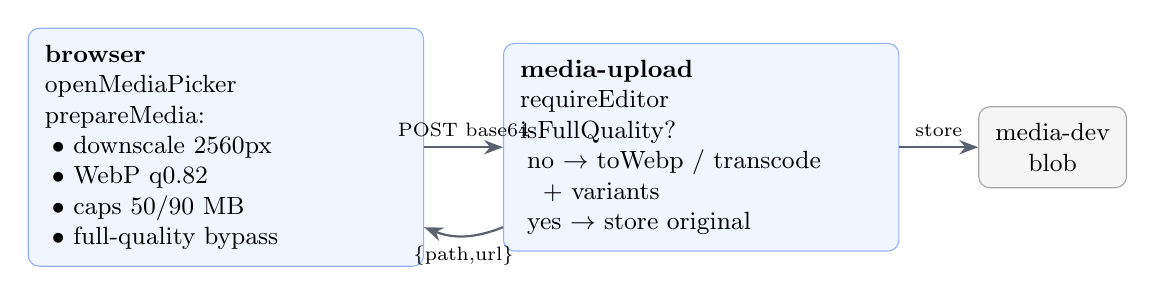
\begin{tikzpicture}[node distance=7mm and 10mm]
  \node[box, align=left, text width=4.6cm] (cli) {\textbf{browser}\\
    openMediaPicker\\ prepareMedia:\\ \;$\bullet$ downscale 2560px\\
    \;$\bullet$ WebP q0.82\\ \;$\bullet$ caps 50/90 MB\\ \;$\bullet$ full-quality bypass};
  \node[box, right=of cli, align=left, text width=4.6cm] (srv) {\textbf{media-upload}\\
    requireEditor\\ isFullQuality?\\ \;no $\to$ toWebp / transcode\\ \;\; + variants\\
    \;yes $\to$ store original};
  \node[gbox, right=of srv] (blob) {media-dev\\ blob};
  \draw[flow] (cli) -- node[above,font=\scriptsize]{POST base64} (srv);
  \draw[flow] (srv) -- node[above,font=\scriptsize]{store} (blob);
  \draw[flow] (srv) to[bend left=22] node[below,font=\scriptsize]{\{path,url\}} (cli);
\end{tikzpicture}
\caption{The upload pipeline; the full-quality rule is mirrored on both ends.}
\end{figure}

%==============================================================================
\section{Publish / Revert and the backend}\label{sec:backend}
%==============================================================================

\subsection{Draft vs published}

Two container sets: \textbf{draft} (\code{content-dev}, \code{media-dev}) --- what
the editor reads and writes --- and \textbf{published} (\code{content-prod},
\code{media-prod}) --- what the live site serves. The editor only ever writes to
draft. Publishing and reverting are server-side copies between the sets.

\subsection{Publish $\to$ /api/promote}

\code{publish()} warns if there are unsaved edits (Publish ships the last
\emph{saved} draft, not in-memory edits), confirms, then POSTs \code{/api/promote},
which copies every content JSON dev\,$\to$\,prod \emph{skipping pages marked}
\code{visibility:'dev'} in \code{global.json} (Dev-only pages never go live), then
syncs media dev\,$\to$\,prod via server-side blob copy from the public-read draft
URL (no bytes flow through the Function).

\subsection{Revert $\to$ /api/revert}

The inverse: copy every content file prod\,$\to$\,dev, restoring the draft to the
last published version, then reload.

\subsection{Auth behind the SWA gate}

Every mutating endpoint calls \code{requireEditor}, reading the
\code{x-ms-client-principal} header that Static Web Apps injects (base64 JSON with
roles) and requiring \code{editor}:

\begin{lstlisting}
// api/_lib/auth.js
function requireEditor(context, req) {
  if (isEditor(req)) return true;   // checks x-ms-client-principal roles
  context.res = { status: 403, body: { error: 'Not authorized - editor role required' } };
  return false;
}
// EDITOR_AUTH_DISABLED=true bypasses this locally (never set in cloud).
\end{lstlisting}

The browser never holds a storage key; the Functions reach blob storage via scoped
per-container SAS tokens in app settings.

\begin{figure}[h]
\centering
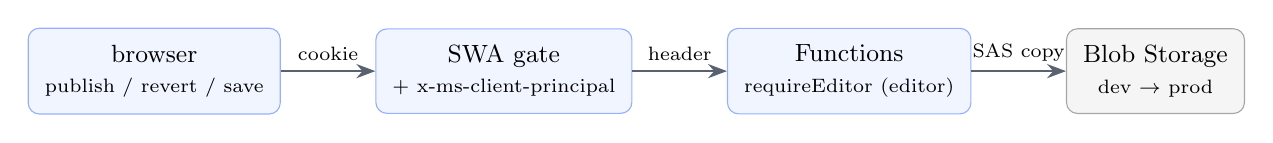
\begin{tikzpicture}[node distance=6mm and 12mm]
  \node[box] (b) {browser\\ \scriptsize publish / revert / save};
  \node[box, right=of b] (swa) {SWA gate\\ \scriptsize + x-ms-client-principal};
  \node[box, right=of swa] (fn) {Functions\\ \scriptsize requireEditor (editor)};
  \node[gbox, right=of fn] (blob) {Blob Storage\\ \scriptsize dev $\to$ prod};
  \draw[flow] (b) -- node[above,font=\scriptsize]{cookie} (swa);
  \draw[flow] (swa) -- node[above,font=\scriptsize]{header} (fn);
  \draw[flow] (fn) -- node[above,font=\scriptsize]{SAS copy} (blob);
\end{tikzpicture}
\caption{Request flow: browser $\to$ SWA $\to$ Functions $\to$ blob.}
\end{figure}

%==============================================================================
\section{How to extend the editor}\label{sec:extend}
%==============================================================================

\subsection{Make a part editable}

You write zero editor code. In your part's render (\code{blocks.js} /
\code{site-blocks.js}), tag the DOM:

\begin{lstlisting}
// inside a part's render(block, ctx)
ctx.el('h2', { 'data-edit-file': ctx.file,
               'data-edit-text': ctx.path + '.title', text: block.title });
ctx.el('img', { 'data-edit-file': ctx.file,
                'data-edit-image': ctx.path + '.src', src: ctx.mediaUrl(block.src) });
var grid = ctx.el('div', { 'data-edit-file': ctx.file,
                           'data-edit-list': ctx.path + '.items',
                           'data-edit-list-label': 'links' });
block.items.forEach(function (it, j) {
  grid.appendChild(ctx.el('a', { 'data-item-index': j, href: it.url, text: it.label })); // stamp j!
});
\end{lstlisting}

\code{bindAll()} discovers and wires these on the next render. Stamp
\code{data-item-index} on filtered lists (\S\ref{sec:list}) and set
\code{data-edit-file} (\S\ref{sec:state}).

\subsection{Add a new inspector field type}

Fields are dispatched by a \code{type} string
(\code{text}, \code{textarea}, \code{url}, \code{image}, \code{bool},
\code{select}, \code{csv}, \code{color}, \code{embed}). To add one, extend the
field-renderer switch with a new \code{case}: build the input, seed it from the
current value via \code{getByPath}, and on change call the supplied
\code{onChange(value)} callback. The case must not write the model directly --- the
callback owns \code{setByPath} + \code{markDirty} + the live re-render. Use the
\code{color} case as a template; it is the most recently added type and shows the
full pattern.

\subsection{Add a panel to the More menu}

Toolbar buttons are built in \code{buildToolbar()}; secondary tools live in the
\code{\#engine-more} dropdown:

\begin{lstlisting}
var btnThing = el('button', { text: 'My Thing', title: '...', on: { click: openThingPanel } });
[btnTheme, btnBg, /* ... */, btnThing].forEach(x => moreMenu.appendChild(x));
\end{lstlisting}

Write \code{openThingPanel()} following the slide-in convention: an
\code{.engine-panel} with an \code{.engine-phead} (title + \code{helpBtn('thing')}
+ Close) and an \code{.engine-pbody}, then \code{panelize()} it into an
\code{.engine-overlay}. Persist with \code{markDirty(state.file)} + \code{save()};
if Done should re-render the page, call \code{save(true)}.

\subsection{The per-tool HELP registry}

Each panel shows a round ``?'' via \code{helpBtn(key)}, opening
\code{openHelpTopic(key)} against the \code{HELP} registry:

\begin{lstlisting}
var HELP = {
  thing: {
    title: 'My Thing',
    intro: 'One sentence on what this does.',
    body: [
      ['A subheading', ['A bullet.', 'Another - note the empty-field behaviour.']]
    ]
  }
  /* sections, pages, theme, style, editsection, lists, questionnaire,
     tracking, background, media, addsection ... */
};
\end{lstlisting}

When you add a panel, add a matching \code{HELP} entry and wire
\code{helpBtn('thing')} into its header. Existing entries are deliberately
plain-language and call out the ``what if I leave this empty?'' edge cases ---
match that tone.

%==============================================================================
\section{Known sharp edges (respect these)}\label{sec:edges}
%==============================================================================

These are real, current behaviours --- things to keep in mind, not to ``fix'' in
passing into a regression.

\begin{enumerate}[leftmargin=1.6em]
  \item \textbf{Unsaved page edits vs Pages-panel navigation.} Inline edits write
  to \code{state.models[pageFile]} and set \code{dirtyFiles}, but are only POSTed
  by \code{save()}. Some navigation flows (Pages ``Open'', create-page, ``Add to
  menu'') run \code{saveGlobal} (persisting only \code{global}) then
  \code{location.href} away --- the dirty \emph{page} model is never saved. The
  \code{beforeunload} guard shows the browser's generic prompt, but it is easy to
  dismiss. New navigation flows should save the page model first (or warn).

  \item \textbf{The staging / live split.} The Sections panel stages changes; the
  page reflects them only after Apply \& Save $\to$ reload. Do not assert against
  the live count mid-edit, and do not add a ``live as you click'' feature without
  reconciling it with \code{applySave}'s built-in/block split.

  \item \textbf{The save $\to$ reload timing.} \code{save(true)} reloads
  $\sim$300--600\,ms later. Anything reading the DOM right after triggering it sees
  stale content. Wait for the reload, or read \code{state.models}.

  \item \textbf{\code{data-edit-html} stores raw contentEditable HTML.} No
  sanitisation; browser-injected \code{<div>}/\code{<br>} and pasted markup are
  persisted. Acceptable for trusted editors; mind it if you widen who can edit.

  \item \textbf{Built-in vs block ordering is not unified} (\S\ref{sec:sections}).

  \item \textbf{Background replace can show a cached old image.} Fixed-blob
  backgrounds reuse the filename; \code{applyLiveBackground} cache-busts the element
  currently showing it, but a stylesheet-rule background can't be repainted and the
  user is told to hard-refresh. Expected, not a bug.

  \item \textbf{The full-quality rule lives in two places} --- client
  \code{SITE.fullQualityMedia} and server \code{MEDIA\_FULL\_QUALITY\_PREFIXES}
  must agree.
\end{enumerate}

\end{document}
